\documentclass[12 pt]{article}

\usepackage{stoversymb}
\usepackage{fullpage,amsmath,amsfonts,amssymb,url,multicol,graphicx,tikz}
%===makes urls render well===
\usepackage{lmodern}
\usepackage[T1]{fontenc}
%============================
\usepackage{wasysym} % smileys
\usepackage[inline]{enumitem}

%,amsthm,amscd,amsbsy,graphpap,makeidx,xfrac,graphicx,floatflt,verbatim,tikz}

%\usetikzlibrary{matrix,arrows}

\everymath{\displaystyle}

\setenumerate{itemsep=0.25in}
\setlist[enumerate,1]{label=\arabic*.}
\setlist[enumerate,2]{label={(\alph*)}}
\setlist[enumerate,3]{label={\roman*.}}

\usepackage{caption,subcaption}
\captionsetup{subrefformat=parens}
\captionsetup{labelformat=simple,justification= centering,labelsep=newline,width=5.5in}
\captionsetup[figure]{belowskip=0px}
\captionsetup*[subfigure]{position=bottom}

\newcommand{\hint}[1]{\hspace{0.5in}\textbf{Hint}: #1}
\newcommand{\graphpaper}{%
	\begin{center}
		
\begin{tikzpicture}
			\draw[step=0.5cm,gray!50,very thin] (-8,-5) grid (8,5);
		\end{tikzpicture}
	\end{center}%
}
\newcommand{\smallgraphpaper}{%
	\begin{center}
		
\begin{tikzpicture}
		\draw[step=0.5cm,gray!50,very thin] (-6,-3.5) grid (6,3.5);
		\end{tikzpicture}
	\end{center}%
}
\newcommand{\polarpaper}[1]{%
	\begin{center}
		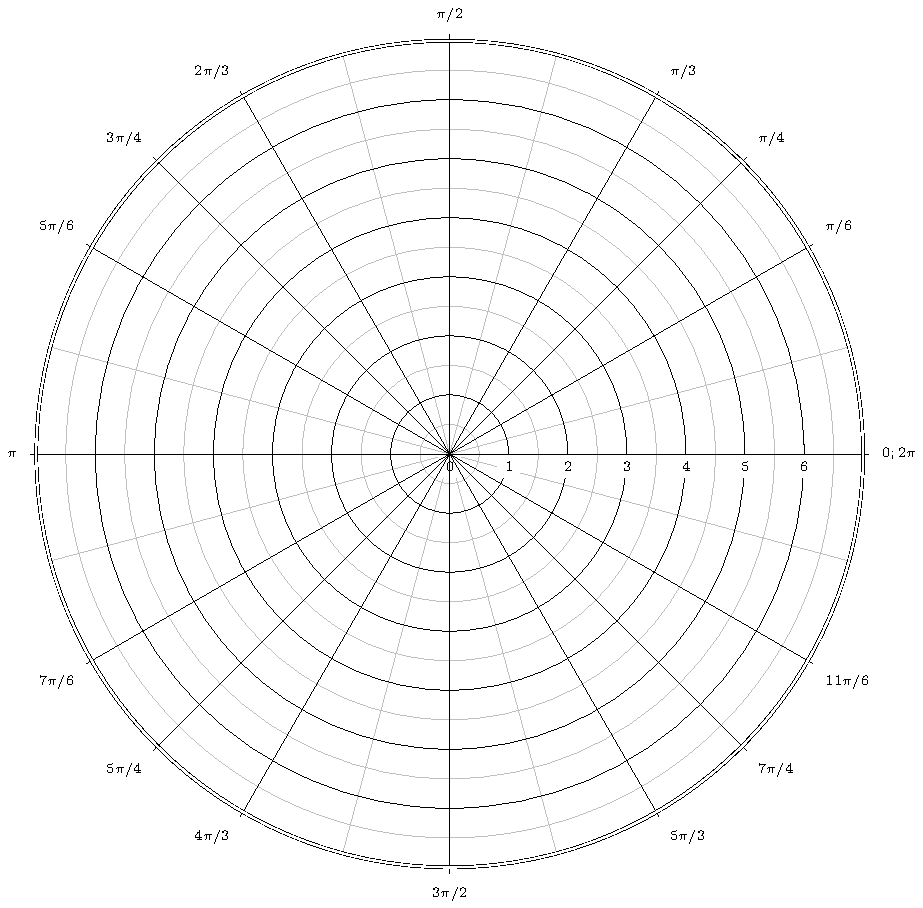
\includegraphics[scale={#1}]{polarpaper}
	\end{center}
}
\newcommand{\smallpolarpaper}[1]{%
	\begin{center}
		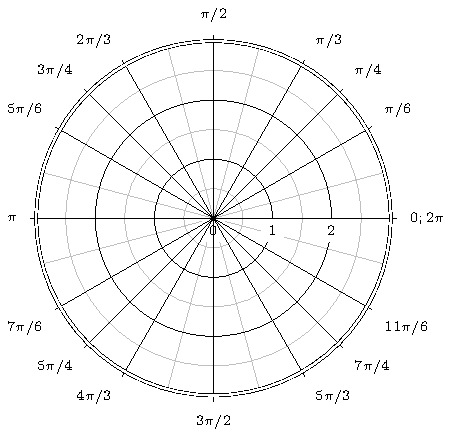
\includegraphics[scale={#1}]{polarpapersmol}
	\end{center}
}

\begin{document}
\begin{flushright}Name: \line(1,0){200}\end{flushright}
\begin{center}
\Large{\textbf{MAC 2312 --- Homework 4}}
\end{center}
\textbf{Directions:} Complete the following problems for a homework grade. Solutions \textit{must} be presented in a neat and professional manner in order to receive credit, answers given without showing work will not be eligible to receive partial credit, and \textit{work for the problems \textbf{must} be done on scratch paper and not on this handout!} \textbf{Date Due:} Tuesday, November 8.
%\vspace{0.0625in}
\begin{enumerate}[leftmargin=0in, rightmargin=-0.25in]
	%========Slack==============
	\item Go to the \#thanksgiving\_st00fs channel in our course's \textsc{Slack} room (see course homepage for the URL) and say something about Thanksgiving. Do you like it? Do you not like it? What do you eat? Are you going somewhere? Tell us things!%\\[3mm]\hint{This is a particularly good exercise to work on improving your test 2 knowledge for possible extra credit things, etc.!}
	%=========Sketch Curve======
	\item Sketch the curve given by the parametric equations $x(t)=t^2$, $y(t)=t^3-4t$, $-4\leq t\leq 4$, by plotting points. Indicate with an arrow the direction in which the curve is traced as $t$ increases.
	\begin{center}
		\renewcommand{\arraystretch}{1.4}
		\begin{tabular}{|c|c|c|c|c|c|c|c|c|c|}
			\hline
			\, $t$ \quad & \quad\quad\quad & \quad\quad\quad & \quad\quad\quad & \quad\quad\quad & \quad\quad\quad & \quad\quad\quad & \quad\quad\quad & \quad\quad\quad & \quad\quad\quad \\
			\hline
			\, $x$ \quad & \quad\quad\quad & \quad\quad\quad & \quad\quad\quad & \quad\quad\quad & \quad\quad\quad & \quad\quad\quad & \quad\quad\quad & \quad\quad\quad & \quad\quad\quad \\
			\hline
			\, $y$ \quad & \quad\quad\quad & \quad\quad\quad & \quad\quad\quad & \quad\quad\quad & \quad\quad\quad & \quad\quad\quad & \quad\quad\quad & \quad\quad\quad & \quad\quad\quad \\
			\hline
		\end{tabular}
	\end{center}
	\graphpaper
	%=========Param Calculus====
	\item Let $C$ be the parametric curve given by $x(t)=\cos(t)$, $y(t)=\sin(t)$, $0~\leq~t<~2\pi$.
	\begin{enumerate}[itemsep=0.375in]
		\item Find $dy/dx$. \textbf{Hint:} You'll want to simplify here.
		\item Find an equation of the tangent line to $C$ at the point $\left(3,e^{16}\right)$.
		\item Find the points on $C$ where the tangent is horizontal or vertical.
		\item Find the intervals on which $C$ is increasing and decreasing.
		\item Find $d^2y/dx^2$. \textbf{Hint:} You'll want to simplify here, too!
		\item Find the intervals on which $C$ is concave up and concave down.
	\end{enumerate}\vspace{0.125in}

	\item Repeat parts (a) through (f) of number 3 for the curve defined by $x(t)=1+\sqrt{t}$, $y(t)=e^{t^2}$.\vspace{0.75in}

	\item Show that the curve $x(t)=t^3-t$, $y(t)=t^2$ has two tangents at $(0,1)$, and sketch its graph.
	
	\smallgraphpaper 
	
	\item Find the area bounded by $y$-axis and the \textit{Lissajous figure} $x(t)=\cos{3t}$, $y(t)=\sin{t}$, $0\leq t\leq 2\pi$ whose graph is shown below.
	
	\begin{center}
		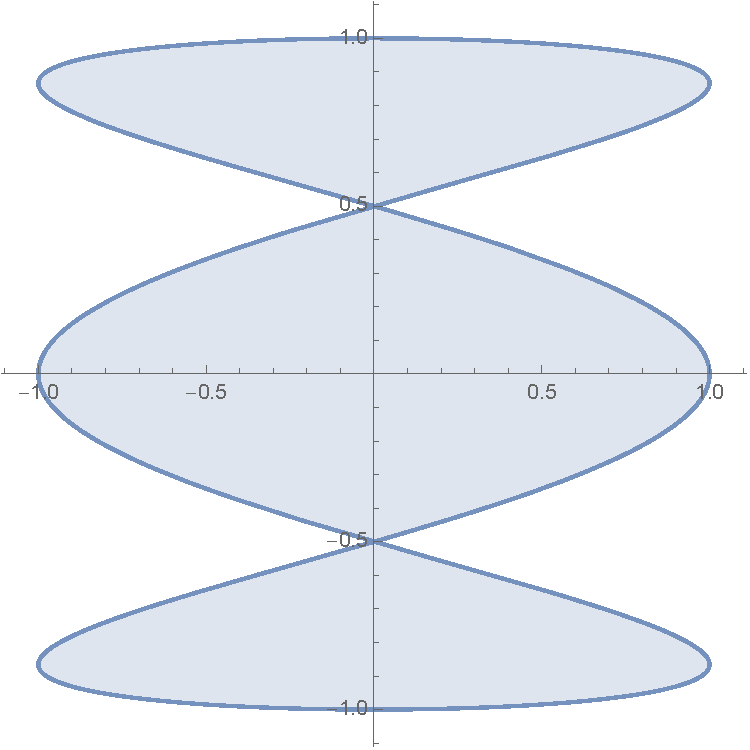
\includegraphics[scale=0.5]{graph5}
	\end{center}
		
	\item Find the length of the curve $x(t)=t^8$, $y(t)=t^4$, $1\leq t\leq 3$. \textbf{Hint: }You'll most likely need $u$-sub \textit{and} trig sub to compute the integral you eventually get, which should look like $$\int_1^3 4t^3\sqrt{(2t^4)^2+1}\,dt\quad\text{(or something equivalent)}.$$
	\vspace{0.25in}
	
	\item \begin{enumerate}[itemsep=0.5in]
		\item Set up an integral that represents the surface area of the solid formed when the portion of the cycloid $x(t)=2(t-\sin{t})$, $y(t)=2(1-\cos{t})$, $0<t<4\pi$, is revolved about the $x$-axis.
		\item Find the exact surface area obtained by rotating the curve $x=2\cos^3{t}$, $y=2\sin^3{t}$, $0\leq t\leq \pi/2$, about the $x$-axis.
	\end{enumerate}\vspace{0.25in}

	\item The \textit{speed} $s$ of a particle $\mathrm{p}$ traveling along the path $x=f(t)$, $y=g(t)$ is defined to be $s~=~\sqrt{[f'(t)]^2+[g'(t)]^2}$. If $\mathrm{p}$ moves around an elliptical track according to the equations $x=\cos{t}$, $y=\sin{2t}$, $0\leq t<2\pi$, when is its speed the greatest? When is it the least?
	\newpage
	%=========Polar Stuff=======
	\item \begin{enumerate}
		\item Plot the points $P_1(5,\pi/6)$, $P_2(-5,\pi/6)$, $P_3(5,\pi/6)$, and $P_4(-5,-\pi/6)$.
		\polarpaper{0.75}
		\item Describe the set of points $P$ whose polar coordinates $(r,\theta)$ satisfy $0\leq r\leq 2$ and $0\leq\theta\leq\pi$.
		\vspace{0.125in}
		\item Convert the following points to polar coordinates: $$\left(2,2\sqrt{3}\right),\quad\left(-2,-2\sqrt{3}\right),\quad(-1,1),\quad(1,-1),\quad(3,7).$$
		\vspace{0.0625in}
		\item Convert the following points to rectangular/Cartesian coordinates: $$\left(3,\pi/4\right),\quad\left(5,-\pi/6\right),\quad(-5,\pi/6),\quad(2,0),\quad(2,3).$$
	\end{enumerate}
	\newpage
	%=========Polar Calculus====
	\item \begin{enumerate}[itemsep=0.75in]
		\item Sketch the curve $r(\theta)=2\sin{2\theta}$. \textbf{Hint:} It should be a rose with some number of petals.
		\smallpolarpaper{1}
		\item Find the equation of the line tangent to $r(\theta)$ at the point $(\sqrt{3},\pi/3)$.
		\item Find the points where the tangent line to the curve $r(\theta)$ are horizontal and/or vertical.
		\item Find the area bounded by the any one petal of the given curve.
		\item Write the integral corresponding to the (arc) length of the portion of the graph of $r(\theta)$ consisting of any \textit{two} petals.
	\end{enumerate}
	\newpage
	\item Find the area of the following shaded region, where the outer curve is given by $r=2+\sin{\theta}$ and where the inner curve is given by $r=\cos(2\theta)$.
	\begin{center}
		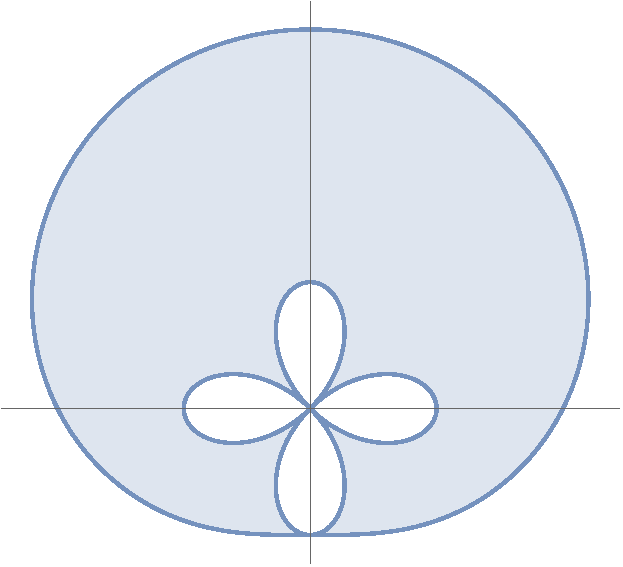
\includegraphics[scale=0.75]{graph2}
	\end{center}
	\item For each of the following, determine \begin{enumerate*}[label=(\roman*)]\item the arc lengths of each of the two curves; and \item the area of the corresponding shaded region. \textbf{Hint:} To find the areas, you'll need to know the intersections of the two curves!
	\end{enumerate*}
	\begin{figure*}[h!]
		\centering
		\begin{subfigure}[t]{0.5\textwidth}
			\centering
			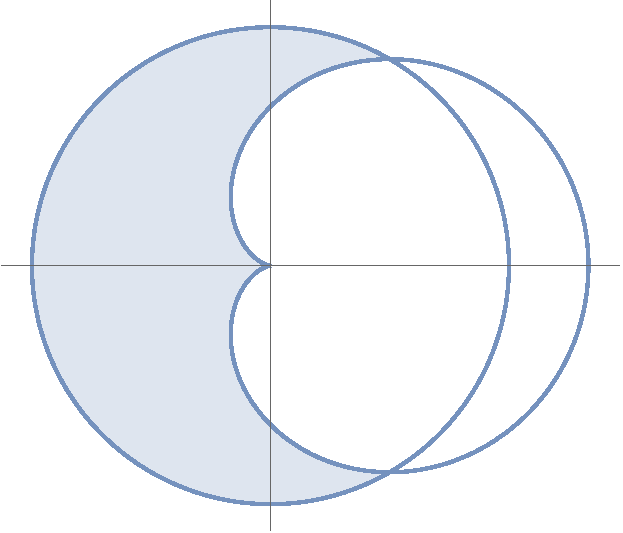
\includegraphics[scale=0.75]{graph3}
			\caption{Circle: $r=3$; Cardioid: $r=2(1+\cos{t})$}
		\end{subfigure}%
		~ 
		\begin{subfigure}[t]{0.5\textwidth}
			\centering
			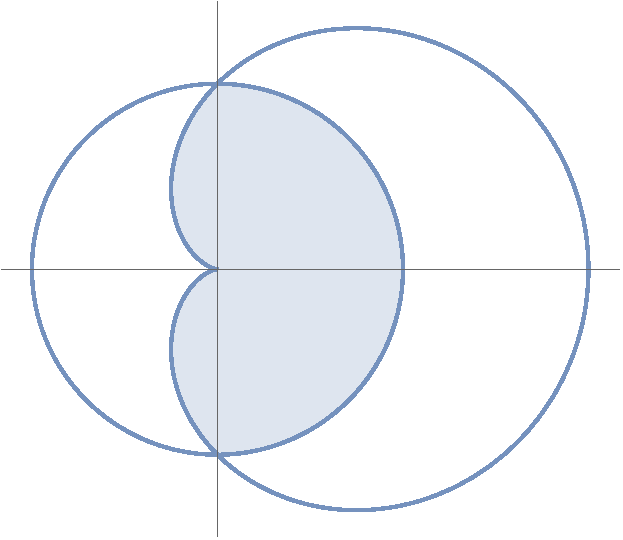
\includegraphics[scale=0.75]{graph4}
			\caption{Circle: $r=1$; Cardioid: $r=1+\cos{t}$}
		\end{subfigure}
	\end{figure*}
\end{enumerate}
\end{document}